\chapter{INTRODUCTION}

\section{Overview}
The Shopify project is a comprehensive digital ecosystem enabling buyers and sellers to interact continuously. Built on the Laravel PHP framework and utilizing React for a dynamic frontend, the system facilitates users to browse products, track orders, and interact with a streamlined seller dashboard.

\section{Objectives}
The primary objective of this project is to create a responsive and scalable e-commerce application. Key goals include:
\begin{itemize}
    \item Deploying a secure and robust authentication system for both buyers and sellers.
    \item Implementing advanced product management, including vector embeddings for algorithmic product recommendations.
    \item Providing real-time user interfaces with minimal payload processing overhead using Inertia.js.
    \item Offering intuitive visual tracking mechanisms for ongoing orders.
\end{itemize}

\section{Scope}
The scope of this web application encompasses front-end user experience (UI/UX) design with Tailwind CSS, a comprehensive relational database schema utilizing Laravel migrations, and backend API integration for various features. 
    
\begin{figure}[H]
    \centering
    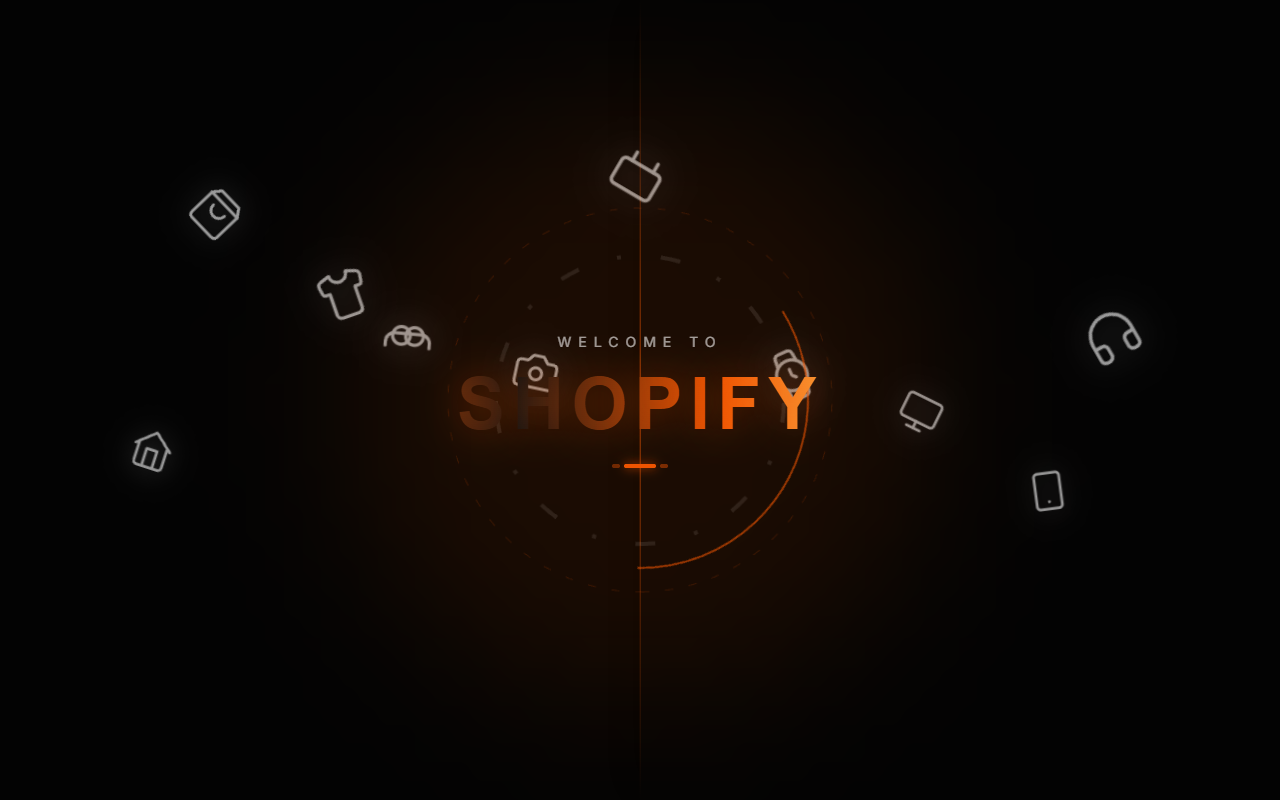
\includegraphics[width=0.8\textwidth]{home.png}
    \caption{Home Page Interface}
    \label{fig:home_page}
\end{figure}
